% options:
% thesis=B bachelor's thesis
% thesis=M master's thesis
% czech thesis in Czech language
% slovak thesis in Slovak language
% english thesis in English language
% hidelinks remove colour boxes around hyperlinks

\documentclass[thesis=B,english]{FITthesis}[2012/06/26]

\usepackage[utf8]{inputenc} % LaTeX source encoded as UTF-8

\usepackage{graphicx} %graphics files inclusion
\usepackage{amsmath} %advanced maths
\DeclareMathOperator*{\argmax}{argmax} % thin space, limits underneath in displays
% \usepackage{amssymb} %additional math symbols

\usepackage{dirtree} %directory tree visualisation

% % list of acronyms
% \usepackage[acronym,nonumberlist,toc,numberedsection=autolabel]{glossaries}
% \iflanguage{czech}{\renewcommand*{\acronymname}{Seznam pou{\v z}it{\' y}ch zkratek}}{}
% \makeglossaries

%\newcommand{\tg}{\mathop{\mathrm{tg}}} %cesky tangens
%\newcommand{\cotg}{\mathop{\mathrm{cotg}}} %cesky cotangens

% % % % % % % % % % % % % % % % % % % % % % % % % % % % % % 
% ODTUD DAL VSE ZMENTE
% % % % % % % % % % % % % % % % % % % % % % % % % % % % % % 

\department{Katedra teoretické informatiky}
\title{Paralelní implementace dynamického naivního Bayesovského klasifikátoru}
\authorGN{Pavel} %(křestní) jméno (jména) autora
\authorFN{Lučivňák} %příjmení autora
\authorWithDegrees{Pavel Lučivňák} %jméno autora včetně současných akademických titulů
\author{Pavel Lučivňák} %jméno autora bez akademických titulů
\supervisor{Ing. Tomáš Šabata}
%\acknowledgements{Doplňte, máte-li komu a za co děkovat. V~opačném případě úplně odstraňte tento příkaz.}
\abstractCS{V~několika větách shrňte obsah a přínos této práce v~češtině. Po přečtení abstraktu by se čtenář měl mít čtenář dost informací pro rozhodnutí, zda chce Vaši práci číst.}
\abstractEN{Sem doplňte ekvivalent abstraktu Vaší práce v~angličtině.}
\placeForDeclarationOfAuthenticity{V~Praze}
\declarationOfAuthenticityOption{4} %volba Prohlášení (číslo 1-6)
\keywordsCS{Nahraďte seznamem klíčových slov v češtině oddělených čárkou.}
\keywordsEN{Nahraďte seznamem klíčových slov v angličtině oddělených čárkou.}
% \website{http://site.example/thesis} %volitelná URL práce, objeví se v tiráži - úplně odstraňte, nemáte-li URL práce

\begin{document}

% \newacronym{CVUT}{{\v C}VUT}{{\v C}esk{\' e} vysok{\' e} u{\v c}en{\' i} technick{\' e} v Praze}
% \newacronym{FIT}{FIT}{Fakulta informa{\v c}n{\' i}ch technologi{\' i}}

\begin{introduction}
	%sem napište úvod Vaší práce
\end{introduction}

\chapter{Cíl práce}

\chapter{Mathematical background}

\section{Probability density function}

Probability density function (PDF) of a continuous random variable determines a likelihood that a given value occurs. Furthermore, \ref{eq:pdf_interval} gives a probability of value being in interval $[a,b]$.

\begin{equation} \label{eq:pdf_interval}
P(a \leq x \leq b) = \int_a^b \text{PDF}(x) dx
\end{equation}

To satisfy the property that $P(-\inf < x < \inf) = 1$, the following has to hold:

\begin{equation}
\int_{-\inf}^{\inf} \text{PDF}(x) dx = 1
\end{equation}

\section{Gaussian distribution}

Gaussian (normal) distribution is defined by a probability density function

\begin{equation} \label{eq:gaussian_pdf}
\text{PDF}_\mathcal{N}(x) = \frac{1}{\sqrt{2 \pi \sigma^2}}e^{-\frac{(x-\mu)^2}{2 \sigma^2}}
\end{equation}

The function is defined by two values - mean $\mu$ and variance $\sigma^2$. Figure \ref{fig:gaussian} provides a visualization of the probability density function.

\begin{figure}
	\centering
 	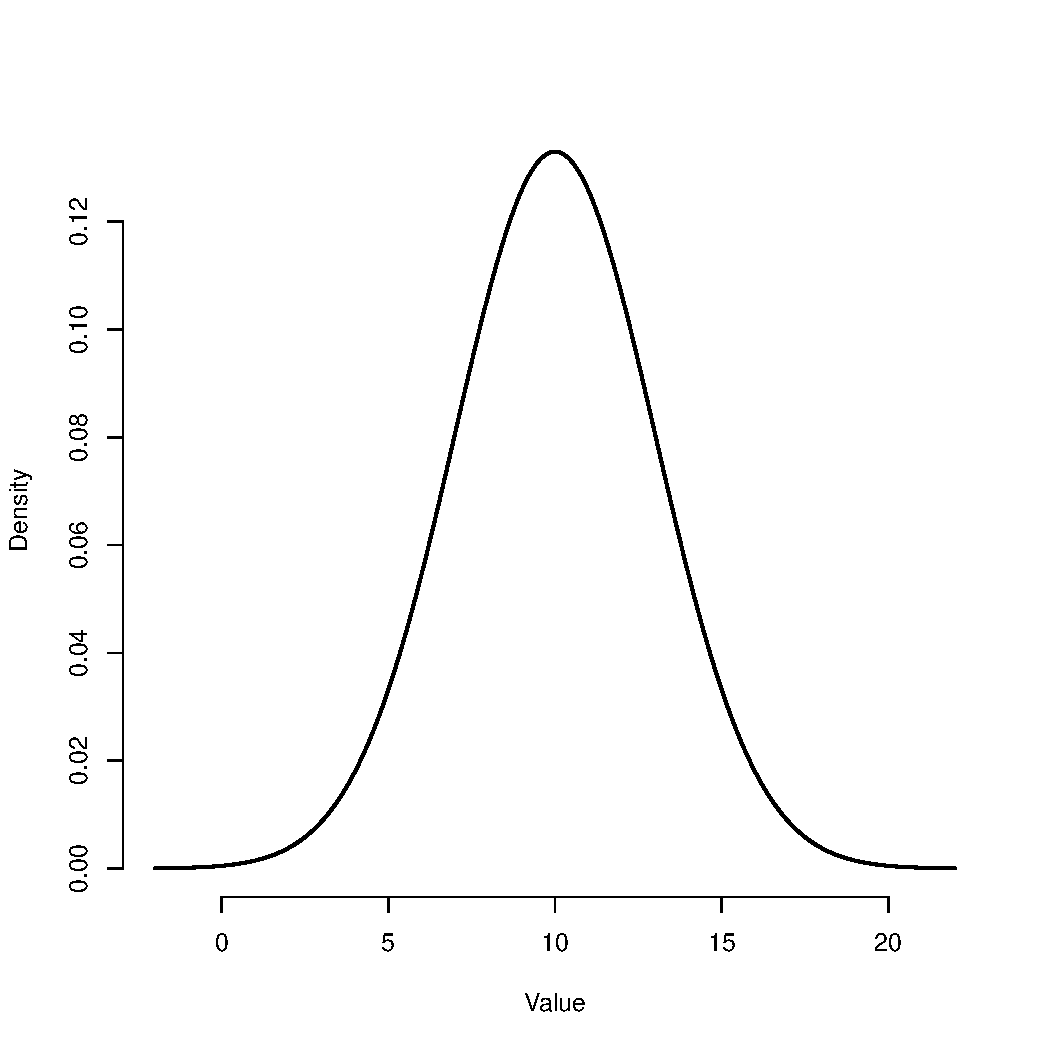
\includegraphics[width=0.7\textwidth]{gaussian}
 	\caption{Visualization of Gaussian PDF with parameters $\mu=10$ and $\sigma^2=3^2$.}
 	\label{fig:gaussian}
\end{figure}

TODO: mention why normal distribution is so important?

\section{Gaussian mixture distribution}

Combining multiple Gaussian distributions together results in Gaussian mixture distribution. The PDF is given by \ref{eq:gaussian_mixture_pdf}, where $n$ is number of mixtures.

\begin{equation} \label{eq:gaussian_mixture_pdf}
\text{PDF}_{\mathcal{N}^*}(x) = \sum_{i=1}^n \text{PDF}_{\mathcal{N}_i}(x)
\end{equation}

\begin{figure}
	\centering
 	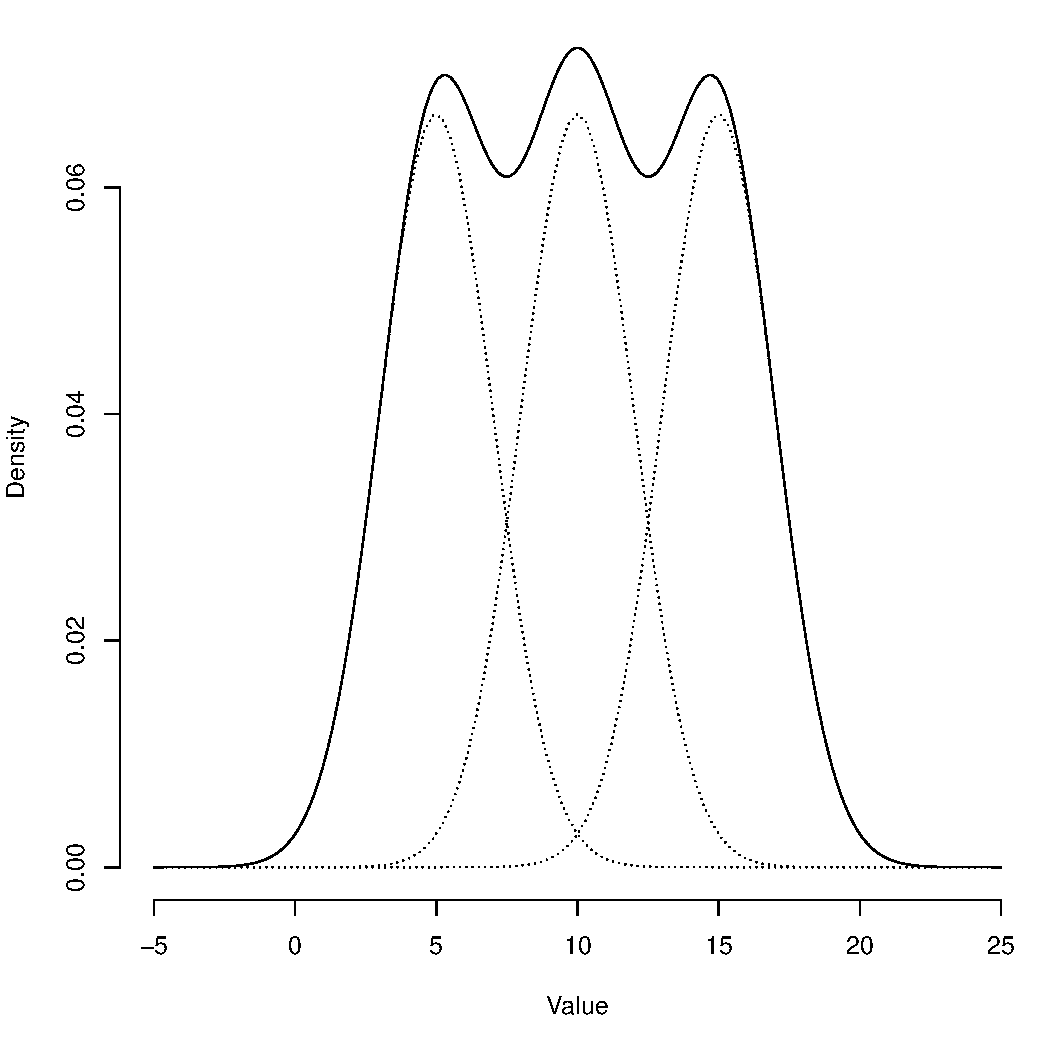
\includegraphics[width=0.7\textwidth]{gaussian_mixture}
 	\caption{Visualization of a mixture of three Gaussian distributions with parameters $\mu_1=5, \mu_2=10, \mu_3=15$ and $\sigma_{1,2,3}^2=2^2$. Author: Smason79, Wikimedia}
 	\label{fig:gaussian_mixture}
\end{figure}

\chapter{Analysis}

\section{Hidden Markov Model}

\subsection{Description}

A Hidden Markov Model (HMM) is defined by
\begin{enumerate}

\item Initial transition function \emph{I}: $S \mapsto \textbf R$
\item Transition function \emph{T}: $S \times S \mapsto \textbf R$ 
\item Emission function \emph{E}: $S \times X \mapsto \textbf R$
\item Set of hidden states \emph{S}
\item Set of observed states \emph{X}

\end{enumerate}

\begin{figure}
	\centering
 	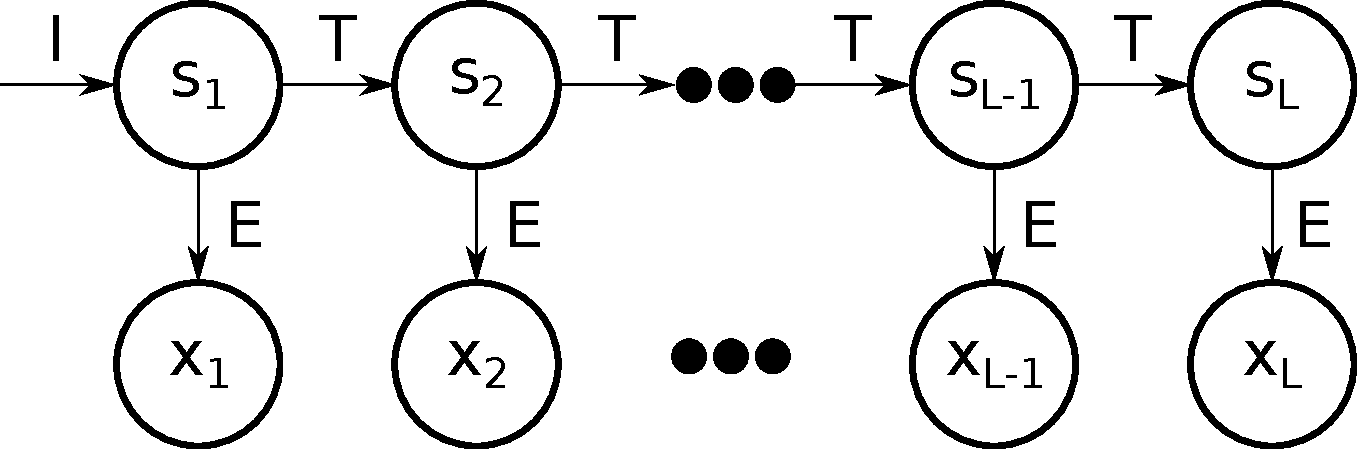
\includegraphics[width=0.7\textwidth]{hmm}
 	\caption{Visualization of a Hidden Markov Model. At each time point, there is a hidden state $s_i$ and an observed state $x_i$.}
 	\label{fig:hmm}
\end{figure}

The aforementioned functions return a probability. This means the resulting number lies in interval $[0, 1]$ and the sum of returned numbers for all function parameters adds to 1.

The set of observed states can be either discrete or continuous. The set of hidden states is assumed to be discrete in the standard definition of HMM.

Given the following:

\begin{enumerate}

\item A number $L \in [1, \inf)$
\item A sequence of hidden states of length \emph{L}
\item A sequence of observed states of length \emph{L}
\item An index \emph{i} $\in [1, L]$: one can think of this as a discrete point in time

\end{enumerate}

At time point \emph{i}, there is a hidden state $s_i$ and an observed state $x_i$. Value of the observed state depends on value of the hidden state. The dependency is described by emission function \emph{E}.

If $i \neq 1$ and $L > 1$, there is a hidden state $s_i$ that depends on value of previous hidden state $s_{i-1}$. The dependency is described by transition function \emph{T}.

If $i = 1$, there is a hidden state $s_1$ that depends on initial transition function \emph{I}.

\subsection{Operations}

There are two most important operations that can be performed on HMM. Learning and inference.

\subsubsection{Learning}

Learning is used to calculate the model parameters $\{I, E, T\} = \lambda$. It is desired to estimate the parameters such that $\prod_{j=1}^{M} P(\textbf x_j | \lambda )$ is maximized. Where $M \in \textbf N$ is a number of sequences to be learned. $\textbf x_j$ is a \emph{j}-th sequence of observed states. In another words, it is desired to maximize the product of probabilities that given sequence of observed states was generated by given model.

\subsubsection{Inference}

Inference returns the most likely sequence of hidden states, given a sequence of observed states.

\subsubsection{Scoring?}

\subsection{Learning}

\subsubsection{Maximum likelihood estimation}

This method uses maximum likelihood estimation (MLE) to compute model parameters. MLE is a technique for finding parameters of a probabilistic model that best describe behavior of a random variable. The method aims to maximize the likelihood of all the learning data.

Formally $\argmax_{\theta \in \Theta} \prod_{j=1}^{M} L(x_j, \theta)$, where:

\begin{itemize}

\item $M$ is number of data points
\item $x_j$ is a j-th data point
\item \emph{L} is a likelihood function (defined further)
\item $\theta$ describes model parameters
\item $\Theta$ is a set of all model parameters

\end{itemize}

Let's examine how one can view parameters of HMM as probabilistic functions of random variables.

\paragraph{Initial transition function}

Function \emph{I}: $S \mapsto \textbf R$ is in fact a probability function corresponding to random variable \emph{S}. To represent it, let's use a discrete probabilistic model with parameter $\epsilon$.

\paragraph{Transition function}

Since the function is $S \times S \mapsto \textbf R$, one can think about it the following way. For each hidden state $s \in S$, there is a probability function $S \mapsto \textbf R$. We can represent such a function in the same way as the initial transition function. Therefore for each hidden state $s \in S$, there is a discrete probabilistic model with parameter $\epsilon$.

\paragraph{Emission function}

Since \emph{E}: $S \times X \mapsto \textbf R$, one can think about it this way. For each hidden state $s \in S$, there is a probability function $X \mapsto \textbf R$. This function can be represented by a continuous probabilistic model. For purposed of this thesis, it is assumed that continuous random variables have Gaussian or Gaussian mixture distribution.

\paragraph{Discrete random variables}

Here I present a straightforward way of defining the $L$ likelihood function in case of discrete random variables. $L(x,\theta) = x_{cnt} / M$, where $x_{cnt}$ is the number of times $x$ occurs in learning data. The number of data points is $M$. Since the likelihood function does not depend on parameter $\theta$, there is no expression to optimize.

There is a reason I did not choose any standard discrete probability distribution to define $L$. The random variable does not have to be \textbf Z, nor \textbf N. In fact it can be any abstract object, such as an animal. A type, where comparison between two objects doesn't make sense. Therefore, it wouldn't make sense to assign non zero probability to values that are not specified in learning phase.

As an example, consider the following data: \{dog, bird, dog, cat, bird, dog\}. Figure \ref{fig:discrete_mle_prob} shows a likelihood function $L$ associated with the data.

% TODO: consider two figures side by side
\begin{figure}
	\centering
 	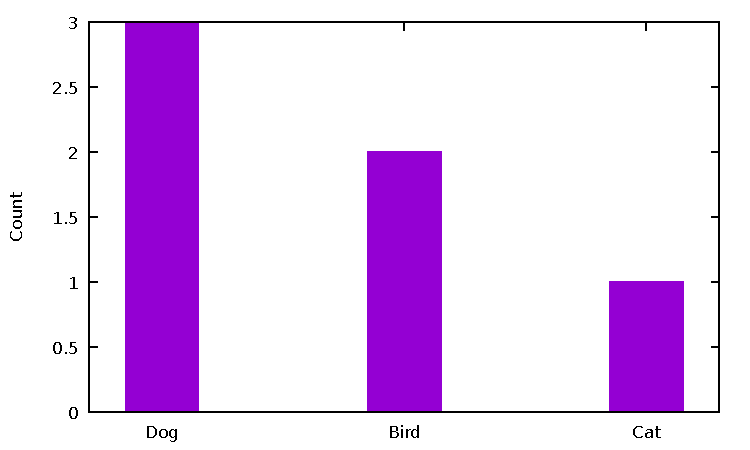
\includegraphics[width=0.7\textwidth]{discrete_mle_hist}
 	\caption{Frequency of data in discrete data set.}
 	\label{fig:discrete_mle_hist}
\end{figure}

\begin{figure}
	\centering
 	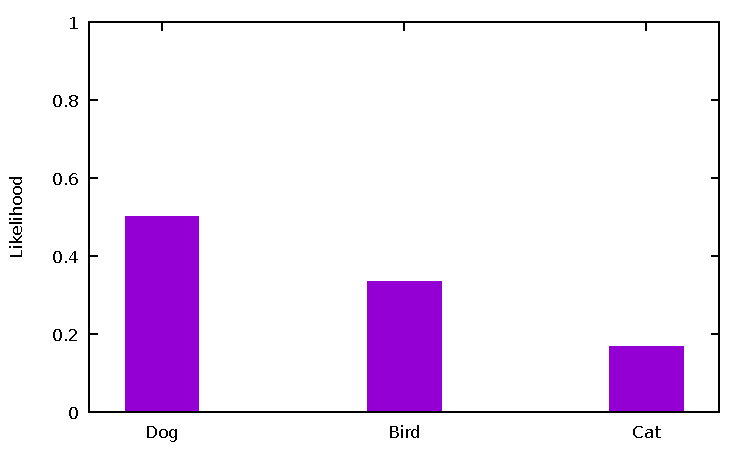
\includegraphics[width=0.7\textwidth]{discrete_mle_prob}
 	\caption{Likelihood function $L$ of data in discrete data set. Probability is zero at undefined states.}
 	\label{fig:discrete_mle_prob}
\end{figure}

\paragraph{Continuous random variables}
% TODO: equations should be on separate lines
Let's consider Gaussian (normal) distribution, defined by $\theta = \{\mu, \sigma^2\}$. The goal is to find parameter $\theta \in \Theta$, such that the product $\prod_{j=1}^{M} L(x_j, \theta)$ is maximized. In case of Gaussian distribution, the likelihood function $L$ is defined by $\frac{1}{\sqrt{2 \pi \sigma^2}}e^{-\frac{(x-\mu)^2}{2 \sigma^2}}$.

Taking derivative with respect to $\mu$ equal to 0 yields $\sum_{j=1}^{M}{x_j - M \mu} = 0$. Maximum likelihood estimate of $\mu$ is therefore equal to $\overline X_M$.

Derivative with respect to $\sigma^2$ equal to zero results in MLE of $\sigma^2$ to be equal to $\frac{1}{M} \sum_{j=1}^{M} {(X_j-\overline X_M)^2}$.

Figure \ref{fig:normal_mle} shows an example of MLE on normally distributed random variable.

\begin{figure}
	\centering
 	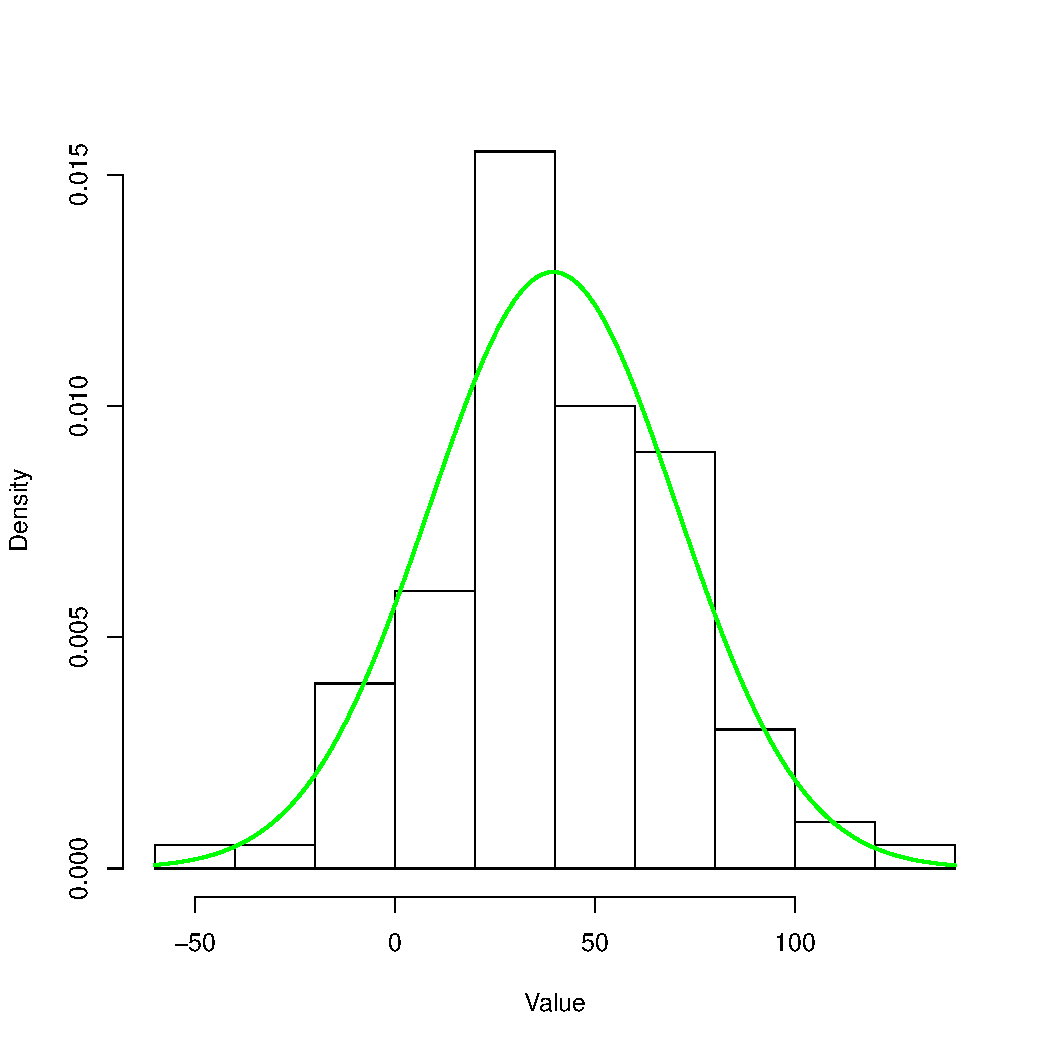
\includegraphics[width=0.7\textwidth]{normal_mle}
 	\caption{Histogram of randomly generated data from normal distribution $\mathcal{N}(40,32^2)$. The green curve is a plot of normal distribution with the maximum likelihood estimate of $\theta$ parameters.}
 	\label{fig:normal_mle}
\end{figure}

TODO: Gaussian mixtures 

\subsection{Inference}

Given a sequence of observed states, what is the most likely associated sequence of hidden states? Viterbi algorithm answers this question. Let's define $a_t(i)$ to be the maximum probability of sequence of hidden and observed states up to time point $t$:

\begin{equation} \label{eq:hmm_viterbi_a}
a_t(i) = max_{s_1,s_2,\dots,s_{t-1}} P(s_1,s_2,\dots,s_{t-1},s_t = S_i,x_1,x_2,\dots,x_t | \theta)
\end{equation}

Where $S_i$ is a function $\textbf N \mapsto S$, assigning a unique index to each hidden state in $S$. $\theta$ are parameters of HMM model.

\paragraph{Initialization}

At time point $t=1$, the probability of being at hidden state $S_i$ is simply the initial probability of being at that state and a probability of being at observed state $x_1$ given hidden state $S_i$. In another words:

\begin{equation}
a_1(i) = I(S_i)E(S_i,x_1)
\end{equation}

\paragraph{Recursion}
Taking into account the structure of HMM, the equation \ref{eq:hmm_viterbi_a} can be rewritten recursively as

\begin{equation} \label{eq:hmm_viterbi_a_rec}
a_t(j) = [\max_i a_{t-1}(i)T(S_i,S_j)] E(S_j,x_t)
\end{equation}

Hidden state at particular time point $t$ is determined by

\begin{equation}
s_t = S_{\argmax_i a_{t}(i)}
\end{equation}

\paragraph{Complexity}

At each time point $t$ and hidden state index $j$, the equation \ref{eq:hmm_viterbi_a_rec} loops through every hidden state index $i$. There are $\vert{S}\vert$ hidden states. In addition, the recursion continues for every time point $t$. There are $L$ time points. Thus the overall complexity is
${\vert{S}\vert}^2 L$.

\section{Dynamic naive Bayesian classifier}

\subsection{Description}

Dynamic naive Bayesian classifier (DNBC) is an extension of Hidden Markov Model (HMM). The difference is that there may be a number of observed variables. In contrast, HMM is defined for only one observed variable. Figure \ref{fig:dnbc} demonstrates model structure with 2 observed variables. DNBC is defined by

\begin{figure}
	\centering
 	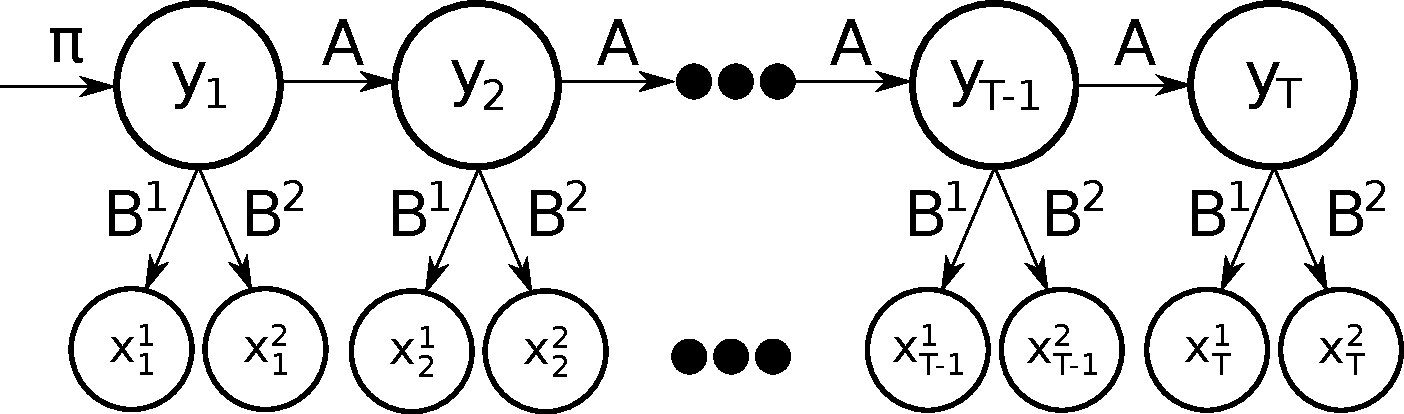
\includegraphics[width=0.7\textwidth]{dnbc}
 	\caption{Visualization of a Dynamic naive Bayesian classifier with two observed variables. At each time point, there is a hidden state $s_i$ and two observed states: $x_i^1$ and $x_i^2$.}
 	\label{fig:dnbc}
\end{figure}

\begin{enumerate}

\item{Number of observed variables $N$}
\item{Initial transition function $I: S \mapsto \textbf R$}
\item{Transition function $T: S \times S \mapsto \textbf R$}
\item{Emission functions $E^j: S \times X^j \mapsto \textbf R, j \in [1,N]$}
\item{Set of hidden states $S$}
\item{Sets of observed states $X^j, j \in [1,N]$}

\end{enumerate}

Each set of observed variables contains a set of observed states. This set can be either discrete or continuous. The set of hidden states is assumed to be discrete.

Given the following:

\begin{enumerate}

\item A number $L \in [1, \inf)$
\item A sequence of hidden states of length \emph{L}
\item Sequences of observed states of length \emph{L}
\item An index \emph{i} $\in [1, L]$: one can think of this as a discrete point in time

\end{enumerate}

At time point \emph{i}, there is a hidden state $s_i$ and $N$ observed states $x^j_i$ where $j \in [1,N]$. Value of every observed state depends on value of the hidden state. The dependency is described by emission function $E^j$. An important property of DNBC is that the observed variables are assumed to be independent. Therefore, DNBC does not define any dependency function between two observed variables.

If $i \neq 1$ and $L > 1$, there is a hidden state $s_i$ that depends on value of previous hidden state $s_{i-1}$. The dependency is described by transition function \emph{T}.

If $i = 1$, there is a hidden state $s_1$ that depends on initial transition function \emph{I}.

\subsection{Operations}

There are two most important operations that can be performed on DNBC. Learning and inference.

\subsubsection{Learning}

Learning is used to calculate the model parameters $\{I,T,E^1,E^2,\dots,E^N\} = \lambda$. It is desired to estimate the parameters such that $\prod_{j=1}^{M} P(\textbf x_j | \lambda )$ is maximized. Where $M \in \textbf N$ is a number of sequences to be learned. $\textbf x_j$ is a \emph{j}-th sequence of observed states. In another words, it is desired to maximize the product of probabilities that given sequence of observed states was generated by given model.

\subsubsection{Inference}

Inference returns the most likely sequence of hidden states, given sequences of observed states. Each sequence of observed states corresponds to particular observed variable. Each sequence thus has the same number of elements.

\subsection{Learning}

\subsubsection{Maximum likelihood estimation}

This learning approach is similar to one described in case of HMM. The only difference is that there are multiple emission functions $E^j$ where $j \in [1,N]$. Every emission function is defined as $E^j: S \times X^j \mapsto \textbf R$. For every $j$ and hidden state $s \in S$, there is a probability function $X^j \mapsto \textbf R$. This function can be represented by continuous probabilistic model. Therefore, there is now $N \times \vert{S}\vert$ continuous distributions to be learned. Each distribution is assumed to be Gaussian or Gaussian mixture.

\subsection{Inference}

Inference algorithm is again Viterbi. It is simply extended to support multiple observed variables. Let $x_t^j$ be a sequence of observed states of variable $j$ up to time point $t$.

\begin{equation}
x_t^j = x_1^j,x_2^j,\dots,x_t^j
\end{equation}

Let's define $a_t(i)$ to be the maximum probability of sequence of hidden and sets of observed states up to time point $t$:

\begin{equation} \label{eq:dnbc_viterbi_a}
a_t(i) = max_{s_1,s_2,\dots,s_{t-1}} P(s_1,s_2,\dots,s_{t-1},s_t = S_i,x_t^1,x_t^2,\dots,x_t^N| \theta)
\end{equation}

Where $S_i$ is a function $\textbf N \mapsto S$, assigning a unique index to each hidden state in $S$. $\theta$ are parameters of DNBC model.

\paragraph{Initialization}

At time point $t=1$, the probability of being at hidden state $S_i$ is equal to the initial probability of being at that state and probabilities of being at observed state $x_1^j$ given hidden state $S_i$. In another words:

\begin{equation}
a_1(i) = I(S_i) \prod_{j=1}^N E^j(S_i,x^j_1)
\end{equation}

\paragraph{Recursion}
Taking into account the structure of DNBC, the equation \ref{eq:dnbc_viterbi_a} can be rewritten recursively as

\begin{equation} \label{eq:dnbc_viterbi_a_rec}
a_t(j) = [\max_i a_{t-1}(i)T(S_i,S_j)] \prod_{k=1}^N E^k(S_j,x^k_t)
\end{equation}

Hidden state at particular time point $t$ is determined by

\begin{equation}
s_t = S_{\argmax_i a_{t}(i)}
\end{equation}

\paragraph{Complexity}

At each time point $t$ and hidden state index $j$, the equation \ref{eq:dnbc_viterbi_a_rec} loops through every hidden state index $i$ and every observed variable index $k$. There are $\vert{S}\vert$ hidden states and $N$ observed variables. In addition, the recursion continues for every time point $t$. There are $L$ time points. Thus the overall time complexity is
${\vert{S}\vert}(\vert{S}\vert+N) L$.

\chapter{Návrh}

\chapter{Realizace}

\begin{conclusion}
	%sem napište závěr Vaší práce
\end{conclusion}

\bibliographystyle{csn690}
\bibliography{mybibliographyfile}

\appendix

\chapter{Seznam použitých zkratek}
% \printglossaries
\begin{description}
	\item[GUI] Graphical user interface
	\item[XML] Extensible markup language
\end{description}

% % % % % % % % % % % % % % % % % % % % % % % % % % % % 
% % Tuto kapitolu z výsledné práce ODSTRAŇTE.
% % % % % % % % % % % % % % % % % % % % % % % % % % % % 
% 
% \chapter{Návod k~použití této šablony}
% 
% Tento dokument slouží jako základ pro napsání závěrečné práce na Fakultě informačních technologií ČVUT v~Praze.
% 
% \section{Výběr základu}
% 
% Vyberte si šablonu podle druhu práce (bakalářská, diplomová), jazyka (čeština, angličtina) a kódování (ASCII, \mbox{UTF-8}, \mbox{ISO-8859-2} neboli latin2 a nebo \mbox{Windows-1250}). 
% 
% V~české variantě naleznete šablony v~souborech pojmenovaných ve formátu práce\_kódování.tex. Typ může být:
% \begin{description}
% 	\item[BP] bakalářská práce,
% 	\item[DP] diplomová (magisterská) práce.
% \end{description}
% Kódování, ve kterém chcete psát, může být:
% \begin{description}
% 	\item[UTF-8] kódování Unicode,
% 	\item[ISO-8859-2] latin2,
% 	\item[Windows-1250] znaková sada 1250 Windows.
% \end{description}
% V~případě nejistoty ohledně kódování doporučujeme následující postup:
% \begin{enumerate}
% 	\item Otevřete šablony pro kódování UTF-8 v~editoru prostého textu, který chcete pro psaní práce použít -- pokud můžete texty s~diakritikou normálně přečíst, použijte tuto šablonu.
% 	\item V~opačném případě postupujte dále podle toho, jaký operační systém používáte:
% 	\begin{itemize}
% 		\item v~případě Windows použijte šablonu pro kódování \mbox{Windows-1250},
% 		\item jinak zkuste použít šablonu pro kódování \mbox{ISO-8859-2}.
% 	\end{itemize}
% \end{enumerate}
% 
% 
% V~anglické variantě jsou šablony pojmenované podle typu práce, možnosti jsou:
% \begin{description}
% 	\item[bachelors] bakalářská práce,
% 	\item[masters] diplomová (magisterská) práce.
% \end{description}
% 
% \section{Použití šablony}
% 
% Šablona je určena pro zpracování systémem \LaTeXe{}. Text je možné psát v~textovém editoru jako prostý text, lze však také využít specializovaný editor pro \LaTeX{}, např. Kile.
% 
% Pro získání tisknutelného výstupu z~takto vytvořeného souboru použijte příkaz \verb|pdflatex|, kterému předáte cestu k~souboru jako parametr. Vhodný editor pro \LaTeX{} toto udělá za Vás. \verb|pdfcslatex| ani \verb|cslatex| \emph{nebudou} s~těmito šablonami fungovat.
% 
% Více informací o~použití systému \LaTeX{} najdete např. v~\cite{wikilatex}.
% 
% \subsection{Typografie}
% 
% Při psaní dodržujte typografické konvence zvoleného jazyka. České \uv{uvozovky} zapisujte použitím příkazu \verb|\uv|, kterému v~parametru předáte text, jenž má být v~uvozovkách. Anglické otevírací uvozovky se v~\LaTeX{}u zadávají jako dva zpětné apostrofy, uzavírací uvozovky jako dva apostrofy. Často chybně uváděný symbol "{} (palce) nemá s~uvozovkami nic společného.
% 
% Dále je třeba zabránit zalomení řádky mezi některými slovy, v~češtině např. za jednopísmennými předložkami a spojkami (vyjma \uv{a}). To docílíte vložením pružné nezalomitelné mezery -- znakem \texttt{\textasciitilde}. V~tomto případě to není třeba dělat ručně, lze použít program \verb|vlna|.
% 
% Více o~typografii viz \cite{kobltypo}.
% 
% \subsection{Obrázky}
% 
% Pro umožnění vkládání obrázků je vhodné použít balíček \verb|graphicx|, samotné vložení se provede příkazem \verb|\includegraphics|. Takto je možné vkládat obrázky ve formátu PDF, PNG a JPEG jestliže používáte pdf\LaTeX{} nebo ve formátu EPS jestliže používáte \LaTeX{}. Doporučujeme preferovat vektorové obrázky před rastrovými (vyjma fotografií).
% 
% \subsubsection{Získání vhodného formátu}
% 
% Pro získání vektorových formátů PDF nebo EPS z~jiných lze použít některý z~vektorových grafických editorů. Pro převod rastrového obrázku na vektorový lze použít rasterizaci, kterou mnohé editory zvládají (např. Inkscape). Pro konverze lze použít též nástroje pro dávkové zpracování běžně dodávané s~\LaTeX{}em, např. \verb|epstopdf|.
% 
% \subsubsection{Plovoucí prostředí}
% 
% Příkazem \verb|\includegraphics| lze obrázky vkládat přímo, doporučujeme však použít plovoucí prostředí, konkrétně \verb|figure|. Například obrázek \ref{fig:float} byl vložen tímto způsobem. Vůbec přitom nevadí, když je obrázek umístěn jinde, než bylo původně zamýšleno -- je tomu tak hlavně kvůli dodržení typografických konvencí. Namísto vynucování konkrétní pozice obrázku doporučujeme používat odkazování z~textu (dvojice příkazů \verb|\label| a \verb|\ref|).
% 
% \begin{figure}\centering
% 	
\includegraphics[width=0.5\textwidth, angle=30]{cvut-logo-bw}
% 	\caption[Příklad obrázku]{Ukázkový obrázek v~plovoucím prostředí}\label{fig:float}
% \end{figure}
% 
% \subsubsection{Verze obrázků}
% 
% % Gnuplot BW i barevně
% Může se hodit mít více verzí stejného obrázku, např. pro barevný či černobílý tisk a nebo pro prezentaci. S~pomocí některých nástrojů na generování grafiky je to snadné.
% 
% Máte-li například graf vytvořený v programu Gnuplot, můžete jeho černobílou variantu (viz obr. \ref{fig:gnuplot-bw}) vytvořit parametrem \verb|monochrome dashed| příkazu \verb|set term|. Barevnou variantu (viz obr. \ref{fig:gnuplot-col}) vhodnou na prezentace lze vytvořit parametrem \verb|colour solid|.
% 
% \begin{figure}\centering
% 	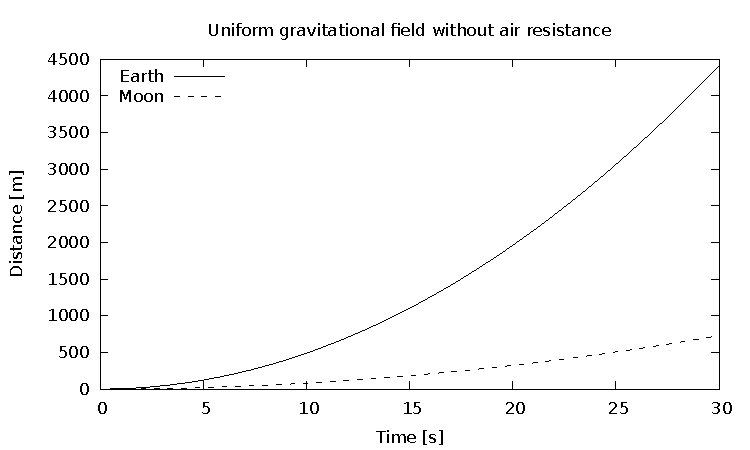
\includegraphics{gnuplot-bw}
% 	\caption{Černobílá varianta obrázku generovaného programem Gnuplot}\label{fig:gnuplot-bw}
% \end{figure}
% 
% \begin{figure}\centering
% 	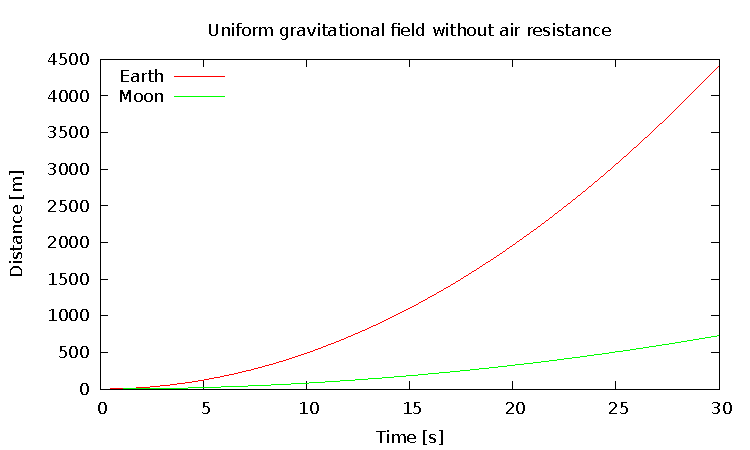
\includegraphics{gnuplot-col}
% 	\caption{Barevná varianta obrázku generovaného programem Gnuplot}\label{fig:gnuplot-col}
% \end{figure}
% 
% 
% \subsection{Tabulky}
% 
% Tabulky lze zadávat různě, např. v~prostředí \verb|tabular|, avšak pro jejich vkládání platí to samé, co pro obrázky -- použijte plovoucí prostředí, v~tomto případě \verb|table|. Například tabulka \ref{tab:matematika} byla vložena tímto způsobem.
% 
% \begin{table}\centering
% 	\caption[Příklad tabulky]{Zadávání matematiky}\label{tab:matematika}
% 	\begin{tabular}{|l|l|c|c|}\hline
% 		Typ		& Prostředí		& \LaTeX{}ovská zkratka	& \TeX{}ovská zkratka	\tabularnewline \hline \hline
% 		Text		& \verb|math|		& \verb|\(...\)|	& \verb|$...$|		\tabularnewline \hline
% 		Displayed	& \verb|displaymath|	& \verb|\[...\]|	& \verb|$$...$$|	\tabularnewline \hline
% 	\end{tabular}
% \end{table}
% 
% % % % % % % % % % % % % % % % % % % % % % % % % % % % 

\chapter{Obsah přiloženého CD}

%upravte podle skutecnosti

\begin{figure}
	\dirtree{%
		.1 readme.txt\DTcomment{stručný popis obsahu CD}.
		.1 exe\DTcomment{adresář se spustitelnou formou implementace}.
		.1 src.
		.2 impl\DTcomment{zdrojové kódy implementace}.
		.2 thesis\DTcomment{zdrojová forma práce ve formátu \LaTeX{}}.
		.1 text\DTcomment{text práce}.
		.2 thesis.pdf\DTcomment{text práce ve formátu PDF}.
		.2 thesis.ps\DTcomment{text práce ve formátu PS}.
	}
\end{figure}

\end{document}
